\documentclass[aspectratio=169,11pt]{beamer}

\usepackage{graphicx}
\usepackage{tikz}
\usetikzlibrary{positioning,arrows.meta}
\usepackage{xcolor}
\usepackage{booktabs}
\usepackage{tabularx}
\usepackage{array}
\usepackage{ragged2e}

\definecolor{GEUBlue}{RGB}{20,55,105}
\definecolor{GEULightBlue}{RGB}{238,244,251}
\definecolor{GEUGrey}{RGB}{90,90,90}
\definecolor{GEULightGrey}{RGB}{245,246,248}

\usetheme{default}
\setbeamertemplate{navigation symbols}{}
\setbeamertemplate{blocks}[rounded][shadow=false]
\setbeamercolor{normal text}{fg=black,bg=white}
\setbeamercolor{frametitle}{fg=GEUBlue}
\setbeamercolor{structure}{fg=GEUBlue}
\setbeamercolor{block title}{fg=GEUBlue,bg=GEULightBlue}
\setbeamercolor{block body}{fg=black,bg=GEULightBlue}
\setbeamerfont{frametitle}{size=\Large,series=\bfseries}

% Keep the same logo convention as the supplied source template.
\newcommand{\GEULogo}{GEU_logo_final.png}

% Header and footer
\setbeamertemplate{headline}{%
  \begin{tikzpicture}[remember picture,overlay]
    \node[anchor=north east,xshift=-0.30cm,yshift=-0.12cm]
      at (current page.north east)
      {\includegraphics[height=0.62cm]{\GEULogo}};
  \end{tikzpicture}
  \vspace{0.72cm}
}
\setbeamertemplate{frametitle}{%
  \vspace{0.03cm}
  \insertframetitle\par
  \vspace{0.04cm}
  \textcolor{GEUBlue}{\rule{\textwidth}{0.9pt}}
  \vspace{0.03cm}
}
\setbeamertemplate{footline}{%
  \leavevmode
  \hbox{%
  \begin{beamercolorbox}[wd=.82\paperwidth,ht=0.32cm,dp=0.10cm,leftskip=.3cm]{author in head/foot}
    \tiny Department of Computer Science \& Engineering | Graphic Era (Deemed to be University)
  \end{beamercolorbox}%
  \begin{beamercolorbox}[wd=.18\paperwidth,ht=0.32cm,dp=0.10cm,rightskip=.3cm]{date in head/foot}
    \hfill\tiny\insertframenumber/\inserttotalframenumber
  \end{beamercolorbox}}
}

\newcommand{\smallnote}[1]{\vspace{0.08cm}{\scriptsize\color{GEUGrey}#1}}

\title{\textbf{Project-Based Learning}\\[2mm]\large Phase-I Evaluation}
\author{\textbf{Campus WiFi Mesh Topology Optimizer}\\Team ID: DSCPP-III-2026-T023}
\institute{Department of Computer Science \& Engineering\\Graphic Era (Deemed to be University), Dehradun}
\date{Academic Session 2026--27}

\begin{document}

% 1
\begin{frame}[plain]
\begin{tikzpicture}[remember picture,overlay]
\draw[GEUBlue,line width=3pt] (current page.north west) -- (current page.north east);
\node[anchor=north east,xshift=-0.45cm,yshift=-0.35cm] at (current page.north east)
{\includegraphics[height=1.0cm]{\GEULogo}};
\node[align=center,text width=.84\paperwidth] at ([yshift=.25cm]current page.center)
{{\color{GEUBlue}\fontsize{26}{30}\selectfont\bfseries PROJECT-BASED LEARNING}\\[3mm]
 {\fontsize{18}{22}\selectfont PHASE-I EVALUATION}\\[7mm]
 {\color{GEUGrey}\Large\bfseries Campus WiFi Mesh Topology Optimizer}\\[3mm]
 {\color{GEUBlue}\normalsize Team ID: DSCPP-III-2026-T023}};
\node[align=center,anchor=south,yshift=.42cm] at (current page.south)
{\bfseries Department of Computer Science \& Engineering\\
Graphic Era (Deemed to be University), Dehradun\\[-1mm]
\scriptsize Academic Session 2026--27};
\end{tikzpicture}
\end{frame}

% 2
\begin{frame}{Team \& Mentor Details}
\begin{columns}[T,totalwidth=\textwidth]
\column{.48\textwidth}
\begin{block}{Team Information}
\begin{tabular}{@{}ll@{}}
\textbf{Team ID:} & DSCPP-III-2026-T023\\
\textbf{Semester:} & 3rd\\
\textbf{Section:} & DS1, DS2, CYBER, ML4\\
\textbf{Domain:} & DSCPP
\end{tabular}
\end{block}

\column{.58\textwidth}
\begin{block}{Team Members}
1.\quad VANSH KAKKAR--2510350011\\
2.\quad SIDDHARTH SHRIDHAR--2510370579\\
3.\quad ANIRUDH RANA--2510011744\\
4.\quad ABHISHEK NEGI--2510380281
\end{block}
\end{columns}

\vspace{2mm}
\begin{block}{Mentor}
\textbf{Dr. Amit Kumar}
\hfill
\textbf{Interactions completed:} 2
\end{block}
\end{frame}

% 3
\begin{frame}{Problem Statement \& Motivation}
\begin{block}{Problem Statement}
Colleges possess numerous WiFi access points; however, improper planning could result in redundant connectivity, interference, increased costs, and inefficient routing. Our project utilizes graph theory algorithms to make the WiFi topology optimal.
\end{block}

\vspace{1mm}
\begin{columns}[T,totalwidth=\textwidth]
\column{.48\textwidth}
\scriptsize
\textbf{\color{GEUBlue}Motivation}
\begin{itemize}\itemsep2pt
\item Lack of simple tools for optimizing WiFi.
\item Causes interference, poor performance, and higher costs.
\item Manual planning is time-consuming and relies on trial and error.
\end{itemize}

\column{.48\textwidth}
\scriptsize
\textbf{\color{GEUBlue}Target Users / Stakeholders}
\begin{itemize}\itemsep2pt
\item Primary Users: Campus network administrators, IT managers running WiFi networks.
\item Secondary stakeholders: Students, faculty, and college management.
\item Expected benefit: Better connectivity.
\end{itemize}
\end{columns}
\end{frame}

% 4
\begin{frame}{Objectives}
\textbf{\color{GEUBlue}Project Objectives}
\vspace{2mm}
\begin{enumerate}\itemsep5pt
\item Improve the campus WiFi network.
\item Limit unnecessary access points.
\item Use Prim's and Kruskal's algorithm.
\item Calculate effective paths using Dijkstra's Algorithm.
\item Compare the network performance before and after optimization.
\end{enumerate}

\vfill
\begin{center}
\colorbox{GEULightBlue}{\parbox{.80\textwidth}{\centering
\textbf{Key Objective:} Lower interference and total network expenses.}}
\end{center}
\end{frame}

% 5
\begin{frame}{Proposed Solution}
\begin{columns}[T,totalwidth=\textwidth]
\column{.48\textwidth}
\scriptsize
\textbf{\color{GEUBlue}Proposed Approach}
\begin{enumerate}\itemsep3pt
\item Collect AP details like distance, latency, bandwidth, and signal strength.
\item Apply Prim's, Kruskal's, and Dijkstra's algorithms.
\item Calculate link costs and select the most efficient connections.
\item Store AP, connection, and network parameter data.
\item Display optimized topology and network performance.
\end{enumerate}

\column{.48\textwidth}
\scriptsize
\textbf{\color{GEUBlue}Key Features}
\begin{itemize}\itemsep3pt
\item Represents APs and connections as a weighted graph.
\item Finds efficient connections while reducing unnecessary links.
\item Uses Prim's, Kruskal's, and Dijkstra's algorithms.
\item Compares latency, interference, cost.
\item Shows the network before and after optimization.
\end{itemize}
\end{columns}

\vspace{3mm}
{\fontsize{4.5}{5.2}\selectfont\color{GEUGrey}\textbf{How it addresses the problem:} The suggested solution uses graph theory to improve WiFi connections, eliminating unnecessary connections, delays, and cost.}
\end{frame}

% 6
\begin{frame}{Integration of PBL Course Concepts}
\scriptsize
\begin{center}
\renewcommand{\arraystretch}{1.25}
\begin{tabularx}{.96\textwidth}{@{}>{\bfseries}p{3.0cm}X p{3.0cm}@{}}
\toprule
Course & Concepts Applied & Project Module\\
\midrule
Data Structures in C & Graphs, Arrays, Linked Lists, Heaps. & Module X: Network Representation and Optimization\\
OOPs with C++ & Classes, Objects, Encapsulation, STL. & Module Y: Network Simulation and Algorithm Implementation\\
\bottomrule
\end{tabularx}
\end{center}

\vfill
\begin{center}
\colorbox{GEULightBlue}{\parbox{.86\textwidth}{\centering
\textbf{Requirement:} Demonstrate meaningful integration of C/C++, OS, and DBMS concepts for network processing, management, and data storage.}}
\end{center}
\end{frame}

% 7
\begin{frame}{System Architecture / Workflow}
\begin{center}
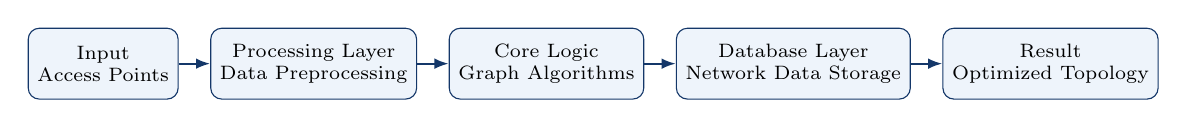
\begin{tikzpicture}[
node distance=4mm,
box/.style={rectangle,rounded corners,draw=GEUBlue,fill=GEULightBlue,
minimum width=1.85cm,minimum height=9mm,align=center,font=\scriptsize},
arrow/.style={-{Latex[length=1.8mm]},thick,draw=GEUBlue}
]
\node[box] (a) {Input\\Access Points};
\node[box,right=of a] (b) {Processing Layer\\Data Preprocessing};
\node[box,right=of b] (c) {Core Logic\\Graph Algorithms};
\node[box,right=of c] (d) {Database Layer\\Network Data Storage};
\node[box,right=of d] (e) {Result\\Optimized Topology};
\draw[arrow] (a)--(b); \draw[arrow] (b)--(c); \draw[arrow] (c)--(d); \draw[arrow] (d)--(e);
\end{tikzpicture}
\end{center}

\vspace{5mm}
\begin{columns}[T,totalwidth=\textwidth]
\column{.48\textwidth}
\textbf{\color{GEUBlue}Major Components}
\begin{itemize}\itemsep2pt
\item Module 1: Network Graph Creation.
\item Module 2: Topology Optimization.
\item Module 3: Route and Performance Analysis.
\end{itemize}

\column{.48\textwidth}
\textbf{\color{GEUBlue}Data / Control Flow}
\begin{itemize}\itemsep2pt
\item Data Flow: AP data $\rightarrow$ preprocessing $\rightarrow$ algorithms $\rightarrow$ output.
\item Modules process data sequentially.
\item Expected Output: Optimized, connected, and efficient WiFi.
\end{itemize}
\end{columns}
\end{frame}

% 8
\begin{frame}{Technology Stack \& Methodology}
\begin{columns}[T,totalwidth=\textwidth]
\column{.48\textwidth}
\begin{block}{Technology Stack}
\scriptsize
\begin{itemize}\itemsep1pt
\item Programming: C / C++
\item Database: File-based storage (CSV / text files).
\item Tools / Framework: VS-Code/Zed/Github
\item IDE: VS-Code/Zed
\item Version Control: Git / GitHub
\end{itemize}
\end{block}

\column{.48\textwidth}
\begin{block}{Development Methodology}
\fontsize{6.2}{7.0}\selectfont
\begin{enumerate}\itemsep0pt
\item \textbf{Requirement Analysis:} Define network optimization needs, access point details, and variables like distance, latency, and signal strength.
\item \textbf{System Design:} Design the Weighted Graph, Data Flow, Algorithms and System Modules.
\item \textbf{Implementation:} Implement graph representation, cost calculation, minimum spanning tree using Prim's or Kruskal's algorithm, and Dijkstra's algorithm in C/Cpp.
\item \textbf{Testing:} Use sample network data for campus to test the system and check connectivity and algorithm results.
\item \textbf{Evaluation:} Compare the network before and after optimization using links, cost, interference, and latency.
\end{enumerate}
\end{block}
\end{columns}

\vfill
\begin{center}
{\tiny\color{GEUGrey}The choice of C/C++ was made for the implementation of data structures and algorithms related to graphs, whereas the use of file-based database gives a simple way to manage the information related to networks. Git/GitHub is used for version control purposes. The use of modular approach of software development was chosen.}
\end{center}
\end{frame}

% 9
\begin{frame}{Initial Progress \& Team Contribution}
\begin{columns}[T,totalwidth=\textwidth]
\column{.44\textwidth}
\scriptsize
\textbf{\color{GEUBlue}Progress Achieved}
\begin{itemize}\itemsep1pt
\item Background/literature study: Research on WiFi mesh networks, graphs, and MST algorithms.
\item Requirements identified: Determined AP information, network specifications, and optimization needs.
\item Architecture prepared: Created the workflow from data input through graph optimization to output.
\item Initial module implemented: Created the base structure of the graph and network optimization component.
\item Database/data preparation: CSV-based file preparation of AP and Network parameters data.
\end{itemize}

\column{.52\textwidth}
\textbf{\color{GEUBlue}Individual Contribution}
\vspace{1mm}
\tiny
\renewcommand{\arraystretch}{1.08}
\begin{tabularx}{\textwidth}{@{}p{2.05cm}p{1.45cm}X@{}}
\toprule
Member & Role & Contribution\\
\midrule
VANSH KAKKAR & Lead & Coordinated the team, finalized project requirements, and worked on the overall system design and work-flow.\\
SIDDHARTH SHRIDHAR & Developer & Worked on graph representation, edge implementation, and development of the core optimization algorithms.\\
ANIRUDH RANA & DB/Testing & Prepared and managed AP/network data using file-based storage and performed testing of the implemented modules.\\
ABHISHEK NEGI & Developer/Docs & Assisted in module development, prepared project documentation, and contributed to the presentation and project report.\\
\bottomrule
\end{tabularx}
\end{columns}
\end{frame}

% 10
\begin{frame}{Roadmap, Expected Outcomes \& References}
\begin{columns}[T,totalwidth=\textwidth]
\column{.47\textwidth}
\scriptsize
\textbf{\color{GEUBlue}Roadmap}
\begin{enumerate}\itemsep3pt
\item Phase-I: Proposal \& Design
\item Phase-II: Development
\item Phase-III: Final Implementation
\end{enumerate}

\vspace{2mm}
\textbf{\color{GEUBlue}Expected Outcomes}
\begin{itemize}\itemsep2pt
\item A simple system to model the WiFi network within the campus and derive its optimal topology.
\item Comparison between the number of connections, cost, and latency before and after optimization.
\item Shows how graph algorithms can help plan efficient WiFi connections.
\item Can be extended to support more APs and larger campus networks.
\end{itemize}

\column{.47\textwidth}
\scriptsize
\textbf{\color{GEUBlue}References}
\begin{enumerate}\itemsep2pt
\item Research papers on WiFi mesh networks and graph-based network topology optimization.
\item Introduction to Algorithms -- Cormen, Leiserson, Rivest \& Stein.
\item Cpp Standard Library and Python/NetworkX documentation.
\item Sample Access Point (AP) and network parameter data prepared for the project, project source code present on GitHub.
\end{enumerate}

\vfill
\begin{center}
\colorbox{GEUBlue}{\parbox{.78\textwidth}{\centering\color{white}\textbf{Thank You}\\Questions \& Suggestions}}
\end{center}
\end{columns}
\end{frame}

\end{document}
